\chapter{Circuito Limitador Básico}
El circuito limitador básico está compuesto por una resistencia en serie y dos Diodos Zener enfrentados, configurados como se observa en la figura \ref{fig:limitador_basico}.

Su propósito es limitar la tensión que emite un circuito de tal manera que este no exceda las tensiones aceptables para un circuito que se encuentre conectado a la salida del regulador. Por ejemplo, en algunos elementos electrónicos no es deseable que la señal de entrada supere los $3.3 \si{\volt}$, y este circuito lo protege de daños por excesos de tensión.

\begin{figure}[ht]
    \begin{center}
        \begin{circuitikz}[american voltages]
    \draw
    (0,0) node[ocirc](Vi-){}
    (0,4) node[ocirc](Vi+){}
    (5,0) node[ocirc](Vo-){}
    (5,4) node[ocirc](Vo+){}
    (Vi+) to[R=$R_s$,-*] ++(3,0)
    to[zzD*, l=$D_{z1}$] ++(0,-2)
    (Vi-) to[short, -*] ++(3,0)
    to[zzD*, l=$D_{z2}$] ++(0,+2)
    (Vo+) -- ++(-2,0)
    (Vo-) -- ++(-2,0)
    (Vi+) to[open, v=$V_i$] (Vi-)
    (Vo+) to[open, v=$V_o$] (Vo-)
    ;
\end{circuitikz}
\caption{Circuito Limitador Básico}
        \label{fig:limitador_basico}
    \end{center}
\end{figure}

\section{Análisis del circuito} \label{sec:limitador_analisis}
Para analizar la operación del circuito se puede pensar en los siguientes casos:

\begin{enumerate}
    \item $|V_i| \leq V_F$
    \item $V_F < |V_i| \leq V_z + V_F$
    \item $V_z + V_F < |V_i|$ 
\end{enumerate}

Dado que los diodos están enfrentados, el comportamiento de este circuito será el mismo tanto para tensiones negativas como positivas.

En el primer caso, como la tensión no es suficiente ni siquiera para polarizar $D_{z1}$, no hay flujo de corriente, por lo tanto la tensión a la salida es $V_o = V_i$. En el segundo caso, la tensión es suficiente para polarizar en directa $D_{z1}$, y $D_{z2}$ se polariza en inversa, pero no alcanza $V_z$ para activarse el modo Zener. Se puede considerar entonces que, dado que la corriente en inversa es despreciable, no hay flujo de corriente y la tensión de salida copia a la de entrada.

En el tercer caso, la tensión de entrada es suficiente para polarizar $D_{z1}$ en directa y en $D_{z2}$ superar la tensión de Zener. Cuando el circuito está operando en esta región, se lo puede interpretar como se observa en la figura \ref{fig:limitador_activado}. A este punto, la salida del circuito estará dada por la expresión \eqref{eqn:transferencia}.

\begin{equation}
    \frac{V_o - (V_F + V_z)}{V_i - (V_F + V_z)}=\frac{r_z}{R_s + r_z}
    \label{eqn:transferencia}
\end{equation}

\begin{figure}[ht]
    \begin{center}
        \begin{circuitikz}[american voltages]
    \draw
    (0,0) node[ocirc](Vi-){}
    (0,4) node[ocirc](Vi+){}
    (5,0) node[ocirc](Vo-){}
    (5,4) node[ocirc](Vo+){}
    (Vi+) to[R=$R_s$,-*] ++(3,0)
    to[battery1, l=$V_F$] ++(0,-2)
    (Vi-) to[short, -*] ++(3,0)
    to [battery1, invert, l=$V_z$] ++(0,1) to[R, resistors/scale=0.5, l=$r_z$] ++(0,1) 
    (Vo+) -- ++(-2,0)
    (Vo-) -- ++(-2,0)
    (Vi+) to[open, v=$V_i$] (Vi-)
    (Vo+) to[open, v=$V_o$] (Vo-)
    ;
\end{circuitikz}
\caption{Circuito Limitador Activado}
        \label{fig:limitador_activado}
    \end{center}
\end{figure}

Debe notarse que, a causa de la impedancia del Diodo Zener en su operación como regulador, la tensión de salida no será constantemente $V_F+V_z$ sino que aumentará a medida que más corriente fluya a través del diodo.

\section{Selección de Componentes}

Se escogió trabajar con el diodo BZX55C3V6, el cual tiene una tensión típica de zener de $V_z = 3.6 \si{\volt}$ y una potencia máxima $P_{max} = 0.5 \si{\watt}$. A partir de estos datos se obtuvo que la corriente máxima que puede circular por el diodo.

\begin{equation}
    I_{max}=\frac{P_{max}}{V_z}
\end{equation}

Luego, la $R_s$ que se debe utilizar estará dada por:

\begin{equation}
    R_{min}=\frac{V_i-(V_z+V_F)}{I_{max}}-r_z
\end{equation}

La mayor $R_{min}$ se obtuvo no tomando la caída de tensión en directa y la resistencia del diodo zener.

\begin{equation}
    R_{min}=\frac{V_i-V_z}{I_{max}}
\end{equation}

Finalmente los componentes y datos obtenidos fueron los siguientes:

\begin{table}[ht]
    \begin{center}
        \begin{tabular}{|l|r|r|r|r|}
            \hline
            Diodo & $V_z$ & $P_{max}$ & $I_{max}$ & $R_{min}$ \\
            \hline
            BZX55C3V6 & $3.6 \si{\volt}$ & $0.5 \si{\watt}$ & $0.139 \si{\ampere}$ & $46.08 \si{\ohm}$ \\
            \hline
        \end{tabular}
        \caption{Restricciones de los componentes del circuito}
        \label{tabla_limitador}
    \end{center}
\end{table}

\begin{table}[ht]
    \begin{center}
        \begin{tabular}{|l|r|r|r|r|}
            \hline
            Diodo & $V_z$ & $r_{\text{z max}}$ & $R_s$ & $V_{\text{F max}}$\\
            \hline
            BZX55C3V6 & $3.6 \si{\volt}$ & $80 \si{\ohm}$ & $100 \si{\ohm}$ & $1.5 \si{\volt}$ \\
            \hline
        \end{tabular}
        \caption{Componentes Utilizados y Características}
    \end{center}
\end{table}

La resistencia fue elegida de modo que el incremento en la caída de tensión, una vez que 
los diodos estén en modo zener, sea bajo. Para las mediciones se utilizó una 
resistencia de $100\Omega$.

\section{Resolución}

\subsection{Teórica}
Teniendo en cuenta los valores de los componentes, y conociendo el comportamiento ideal 
del circuito, se sabe que cuando $|V_i|< V_F+V_z$ la tensión de salida sigue a la entrada.

Fuera de esta región, la recta tendrá una pendiente de $\frac{r_z}{R_s+r_z}$.
\subsection{Simulación}
Se utilizó la siguiente configuración para simular el comportamiento del circuito


\begin{figure}[H]
    \begin{center}
        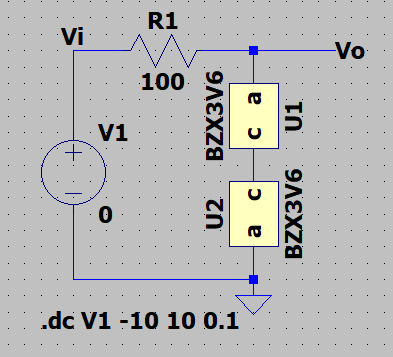
\includegraphics[width=9cm]{limitador/limitador_spice.png}
        \caption{Configuración del circuito en LTSpice XVII}
    \end{center}
\end{figure}

\subsection{Práctica}
Para medir el circuito limitador se implementó el mismo en la protoboard del 
\textit{Electronic Explorer} como se puede ver en la imagen [\ref{implementacion_limitador}].
Se utilizaron tres puntas para medir la tensión en la entrada, en la salida y sobre cada 
diodo. \par 
Se utilizaron scripts para realizar un \textit{DC Sweep} sobre el circuito en el rango 
$\pm 9V$, limitiación impuesta por el equipo.

\begin{figure}[H]
    \begin{center}
        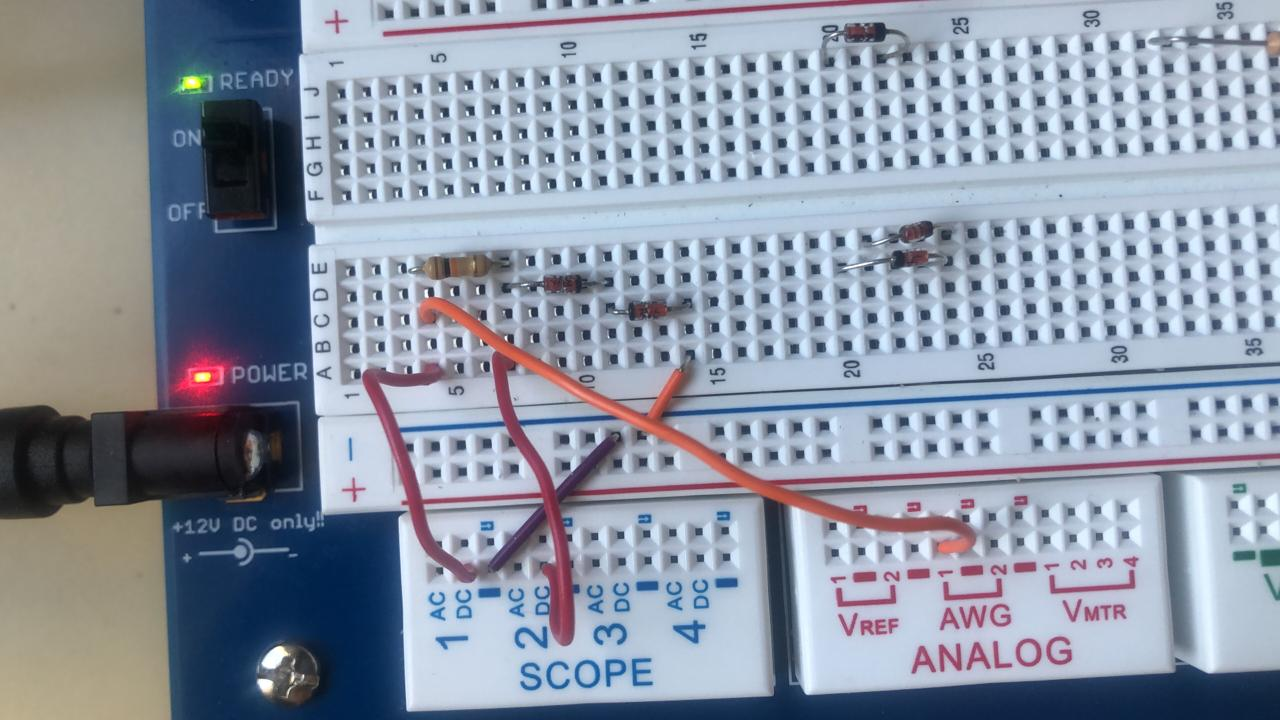
\includegraphics[width=0.7\textwidth]{limitador/Imagenes/foto_medicion_limitador.jpeg}
        \caption{Implementación del circuito}
        \label{implementacion_limitador}
    \end{center}
\end{figure}

\section{Resultados}
Los resultados de todos los desarrollos se representaron en la figura \ref{fig:lim_inout}

\begin{figure}[H]
    \begin{center}
        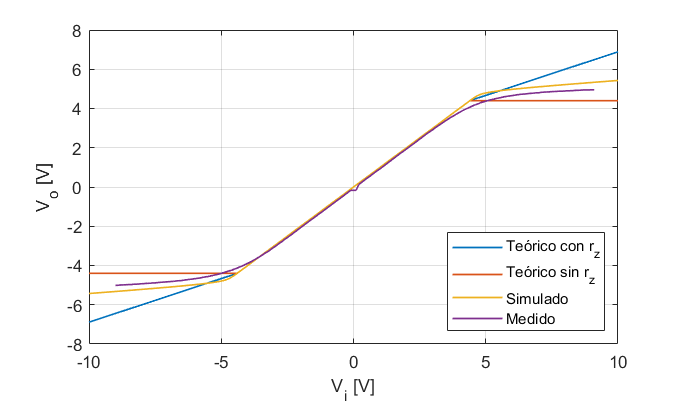
\includegraphics[width=12.7cm]{limitador/Imagenes/limitador_inout.png}
        \caption{Tensión de salida contra tensión de entrada}
        \label{fig:lim_inout}
    \end{center}
\end{figure}

\section{Ganancia de tensión}
Se realizó también el análisis de la ganancia de tensión del circuito limitador. 

Se consideraron dos casos, con y sin $r_z$. En el primer caso, se consideró la $r_z$ de la hoja de datos del fabricante, que toma un valor máximo de $80 \si{\ohm}$.

Como era de esperarse, 
dentro de los dos primeros casos descriptos en la sección 
\ref{sec:limitador_analisis} la ganancia de tensión es unitaria
 en el análisis teórico. Sin embargo, fuera de estas regiones
  esta ganancia ya no es unitaria sino que es dependiente de
   la impedancia del diodo zener. Esto se puede observar 
   claramente en la
    figura \ref{fig:lim_gain}.

\begin{figure}[H]
    \begin{center}
        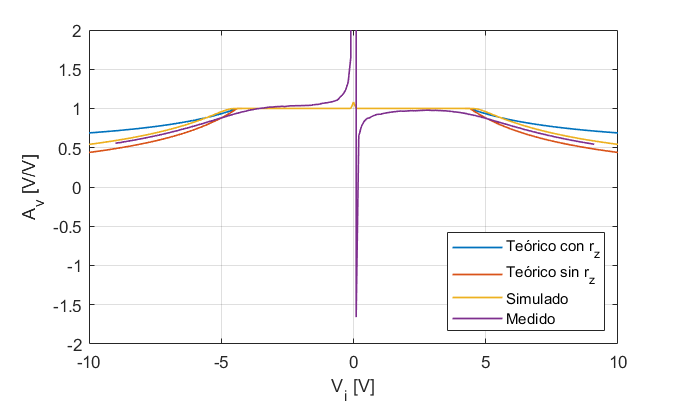
\includegraphics[width=12.7cm]{limitador/Imagenes/limitador_gain.png}
        \caption{Ganancia de tensión contra tensión de entrada}
        \label{fig:lim_gain}
    \end{center}
\end{figure}

Debe notarse que el pico que se observa en el entorno
 de los $0 \si{\volt}$ en la ganancia, 
para el caso de las mediciones, se debe a que los valores medidos 
  son pequeños tal que la función empieza a diverger, debido a que se está dividiendo por 
  cero. En realidad, la ganancia es unitaria siempre que el transistor no esté polarizado, 
  incluído a $0 \si{\volt}$ donde habría tensión nula tanto a la salida como a la entrada.

\section{Variaciones del Circuito}

Utilizando una $R_s$ mayor es posible aplanar aún más la tensión de salida en las exteriores a la zona lineal del circuito.

Al introducir una carga a este circuito, es necesario tener cuidado de que la corriente que fluye entre los diodos no sea tan baja de forma que no sea suficiente para activar el diodo Zener.

\section{Conclusiones}
Se puede observar de los resultados que la salida del circuito medido se encuentra dentro de los márgenes calculados con los datos provistos por la hoja de datos del fabricante. Se puede también observar cómo en la realidad, la entrada a la zona Zener no es abrupta, sino suave. Sin embargo, el aumento de tensión sigue en evidencia a causa de la resistencia del diodo en modo Zener.